
\documentclass{standalone}

\usepackage{pgf}
\usepackage{tikz}
\usetikzlibrary{arrows,automata,matrix}
\usepackage[latin1]{inputenc}
\begin{document}
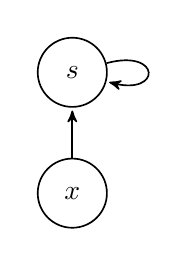
\begin{tikzpicture}[->,>=stealth',shorten >=1pt,auto,node distance=2.8cm,
                    semithick]
  \tikzstyle{every state}=[]

      \matrix (m) [matrix of nodes
      ,row sep=.25in,column sep=.25in] {
      \node[state](s) {$s$}; \\
      \node[state](x) {$x$}; \\
      };
    

  \path (x) edge              node {} (s)
        (s) edge [loop right] node {} (s);
 
\end{tikzpicture}

\end{document}